\chapter{Fundamental Group}
The fundamental group connects topology and algebra together. To get an intuition about the fundamental group of a topological space, consider the example \({S}^{2}\) (2-sphere) and \(\mathbb{T} ={S}^{1} \times  {S}^{1}\) (torus). Pictorially, all loops in $S^2$ be contracted into a point:
\begin{center}
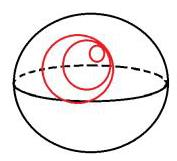
\includegraphics[width=0.3\textwidth]{images/Ch7_S2.jpg}
\end{center}
while some loops in the torus cannot be contracted into a point:
\begin{center}
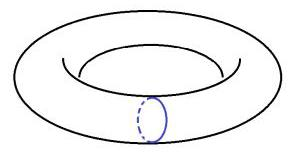
\includegraphics[width=0.3\textwidth]{images/Ch7_T.jpg}
\end{center}
In this chapter, we will use groups to describe this phenomenon formally.


\begin{definition} [loop] Let \(X\) be a topological space. A \emph{loop} on \(X\) is a constant map \(\ell  : \left\lbrack  {0,1}\right\rbrack   \rightarrow  X\) such that \(\ell \left( 0\right)  = \ell \left( 1\right)\).

We say \(\ell\) is \emph{based at \(b \in  X\)} if \(\ell \left( 0\right)  = \ell \left( 1\right)  = b\).
\end{definition}

\begin{definition} [composite loop] Suppose that \(\mathbf{u},\mathbf{v}\) are loops on \(X\) based at \(b \in  X\). The composite loop \(u \cdot  v\) is given by
\[
u \cdot  v = \left\{  \begin{array}{rr} u\left( {2t}\right), & \text{ if }0 \leq  t \leq  1/2 \\  v\left( {{2t} - 1}\right), & \text{ if }1/2 \leq  t \leq  1 \end{array}\right.
\]
\end{definition}

\begin{definition} \label{def:fund_group} [fundamental group] The homotopy class of loops relative to \(\{ 0,1\}\) based at \(b \in  X\) forms a group. It is called the fundamental group of \(X\) based at \(b\), denoted as \({\pi }_{1}\left( {X,b}\right)\).

More precisely, let
\begin{center}
\(\left\lbrack  \ell \right\rbrack   = \{ m \mid  m\) is a loop based at \(b\) that is homotopic to \(\ell\), relative to \(\{ 0,1\} \}\)\end{center}
Then 
\begin{center} \({\pi }_{1}\left( {X,b}\right)  := \{ \left\lbrack  \ell \right\rbrack   \mid  \ell\) are loops based at \(b\}\).\end{center} 
The multiplication operation in \({\pi }_{1}\left( {X,b}\right)\) is defined as:
\[
\left\lbrack  \ell \right\rbrack   * \left\lbrack  {\ell }^{\prime }\right\rbrack   \mathrel{\text{ := }} \left\lbrack  {\ell  \cdot  {\ell }^{\prime }}\right\rbrack ,\;\forall \left\lbrack  \ell \right\rbrack ,\left\lbrack  {\ell }^{\prime }\right\rbrack   \in  {\pi }_{1}\left( {X,b}\right).
\]
\end{definition}

Recall that two paths \({\ell }_{1},{\ell }_{2} : \left\lbrack  {0,1}\right\rbrack   \rightarrow  X\) are homotopic {\bf relative to} \(\{ 0,1\}\) if we can find \(H : \left\lbrack  {0,1}\right\rbrack   \times  \left\lbrack  {0,1}\right\rbrack   \rightarrow  X\) such that
\[
H\left( {t,0}\right)  = {\ell }_{1}\left( t\right),\;H\left( {t,1}\right)  = {\ell }_{2}\left( t\right)
\]
and
\[
H\left( {0,s}\right)  = {\ell }_{1}\left( 0\right)  = {\ell }_{2}\left( 0\right),\forall 0 \leq  s \leq  1,\;H\left( {1,s}\right)  = {\ell }_{1}\left( 1\right)  = {\ell }_{2}\left( 1\right),\forall 0 \leq  s \leq  1.
\]
For instance, the following picture denotes a homotopy of $\ell_1$ and $\ell_2$ {\bf not} relative to \(\{ 0,1\}\) :
\begin{center}
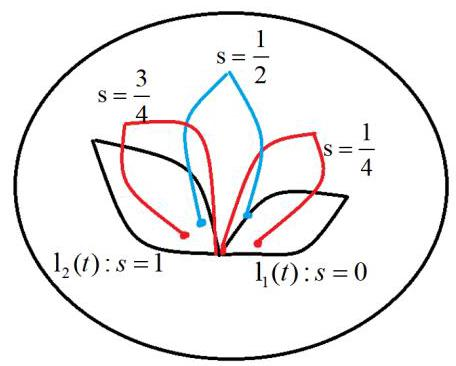
\includegraphics[width=0.36\textwidth]{images/Ch7_not_relative_boundary.jpg}
\end{center}
And below is a homotopy relative to \(\{ 0,1\}\):
\begin{center}
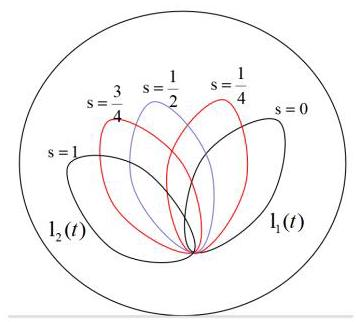
\includegraphics[width=0.36\textwidth]{images/Ch7_relative_boundary.jpg}
\end{center}

It is essential to study homotopy relative to \(\{ 0,1\}\). For example, given a torus with a loop \({\ell }_{1}\left( t\right)\) and a base point \(b\). We want to distinguish \({\ell }_{1}\left( t\right)\) and \({\ell }_{2}\left( t\right)\):
\begin{center}
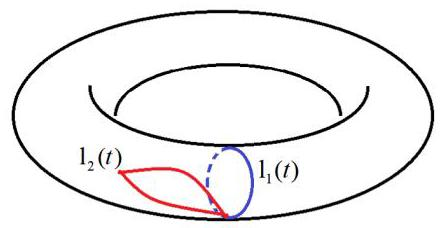
\includegraphics[width=0.4\textwidth]{images/Ch7_2_loops_on_T.jpg}
\end{center}
Obviously, there should be something different between \({\ell }_{1}\left( t\right)\) and \({\ell }_{2}\left( t\right)\). However, if we get rid of this `relative' condition, all loops are homotopic to the constant map \({c}_{b}\left( t\right)  = b\):
\begin{center}
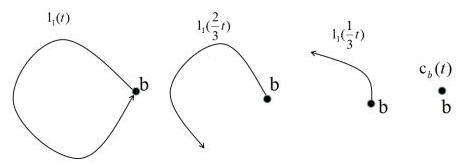
\includegraphics[width=0.5\textwidth]{images/Ch7_homotopic_to_constant.jpg}
\end{center}
In this case, \(\ell  \simeq  {c}_{b}\) for any loop \(\ell\). As a result, there is only one trivial element \(\left\{  \left\lbrack  {c}_{b}\right\rbrack  \right\}\) in \({\pi }_{1}\left( {X,b}\right)\).

That’s the reason why we define \({\pi }_{1}\left( {X,b}\right)\) as the collection of homotopy classes relative to \(\{ 0,1\}\) based at \(b\) in \(X\), so that the continuous deformations of $\ell_1$ are all loops based at $b$.

Now we need to show that the multiplication we defined in \autoref{def:fund_group} does give a group structure of $\pi_1(X,b)$:
\begin{theorem} \label{thm:pi1_forms_a_group} Let \(\left\lbrack  \cdot \right\rbrack\) denote the homotopy class of loops relative to \(\{ 0,1\}\) based at \(b\), and define the operation
\[
\left\lbrack  \ell \right\rbrack   * \left\lbrack  {\ell }^{\prime }\right\rbrack   = \left\lbrack  {\ell  \cdot  {\ell }^{\prime }}\right\rbrack
\]
Then \(\left( {{\pi }_{1}\left( {X,b}\right), * }\right)\) forms a group, where
\[
{\pi }_{1}\left( {X,b}\right)  \mathrel{\text{ := }} \{ \left\lbrack  \ell \right\rbrack   \mid  \ell  : \left\lbrack  {0,1}\right\rbrack   \rightarrow  X\text{ denotes loops based at }b\}
\]
\end{theorem}

\begin{proof} 1. Well-definedness: Suppose that \(u \sim  {u}^{\prime }\) and \(v \sim  {v}^{\prime }\), it suffices to show \(u \cdot  v \simeq\)  \({u}^{\prime } \cdot  {v}^{\prime }\). Consider the given homotopies \(H : u \simeq  {u}^{\prime },K : v \simeq  {v}^{\prime }\). Construct a new homotopy \(L : I \times  I \rightarrow  X\) by

\[
L\left( {t,s}\right)  = \left\{  \begin{array}{rr} H\left( {{2t},s}\right), & 0 \leq  t \leq  1/2 \\  K\left( {{2t} - 1,s}\right), & 1/2 \leq  t \leq  1 \end{array}\right.
\]

The diagram below explains the ideas for constructing \(L\). The plane denote the set \(I \times  I\), and the labels characterize the images of each point of \(I \times  I\) under \(L\). 
\begin{center}
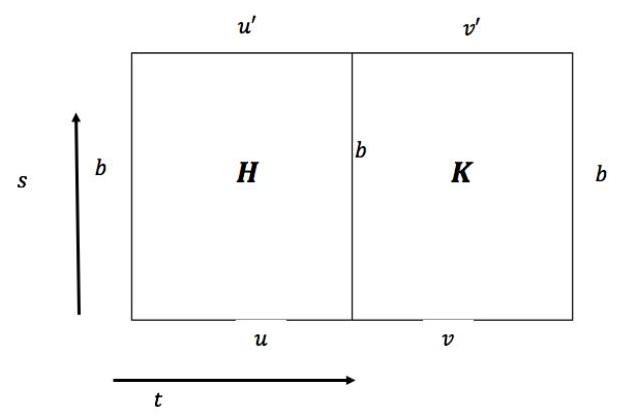
\includegraphics[width=0.6\textwidth]{images/Ch7_well_defined_pi1.jpg}
\end{center}
Therefore, \(u \cdot  v \simeq  {u}^{\prime } \cdot  {v}^{\prime }\).

2. Associativity: Note that \(\left( {u \cdot  v}\right)  \cdot  w\) and \(u \cdot  \left( {v \cdot  w}\right)\) are essentially different loops. Although they go with the same path, they are with different speeds. More explicitly, the loop \(\left( {u \cdot  v}\right)  \cdot  w\) travels \(u,v\) using \(1/4\) seconds, and \(w\) in \(1/2\) seconds; but the loop \(u \cdot  \left( {v \cdot  w}\right)\) travels \(u\) in \(1/2\) seconds, and then \(v,w\) in \(1/4\) seconds.

We want to construct a homotopy that describes the loop changes from \(u \cdot  \left( {v \cdot  w}\right)\) to \(\left( {u \cdot  v}\right)  \cdot  w\). A graphic illustration is given below:
\begin{center}
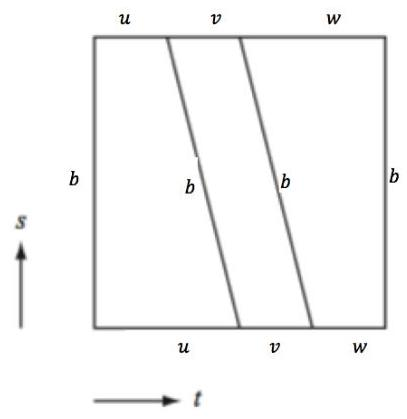
\includegraphics[width=0.5\textwidth]{images/Ch7_associativity_pi1.jpg}
\end{center}
More explicitly, the homotopy \(H : I \times  I \rightarrow  X\) is given by:
\[
H\left( {t,s}\right)  = \left\{  \begin{matrix} u\left( {{4t}/\left( {2 - s}\right) }\right), & 0 \leq  t \leq  1/2 - 1/{4s} \\  v\left( {{4t} - 2 + s}\right), & 1/2 - 1/{4s} \leq  t \leq  3/4 - 1/{4s} \\  w\left( {{4t} - 3 + s/\left( {1 + s}\right) }\right), & 3/4 - 1/{4s} \leq  t \leq  1 \end{matrix}\right.
\]
Therefore,
\[
\left\lbrack  u\right\rbrack   * \left( {\left\lbrack  v\right\rbrack   * \left\lbrack  w\right\rbrack  }\right)  = \left( {\left\lbrack  u\right\rbrack   * \left\lbrack  v\right\rbrack  }\right)  * \left\lbrack  w\right\rbrack
\]

3. Identity: The identity element is the constant map, i.e., let \({c}_{b} : I \rightarrow  X\) by \({c}_{b}\left( t\right)  =b,\forall t\), and let \(e  = \left\lbrack  {c}_{b}\right\rbrack\). Then it suffices to show
\[
e * \left\lbrack  \ell \right\rbrack   = \left\lbrack  \ell \right\rbrack   * e  = \left\lbrack  \ell \right\rbrack   \Leftrightarrow  \left\lbrack  {{c}_{b} \cdot  \ell }\right\rbrack   = \left\lbrack  {\ell  \cdot  {c}_{b}}\right\rbrack   = \left\lbrack  \ell \right\rbrack
\]
Or equivalently,
\[
{c}_{b} \cdot  \ell  \simeq  \ell,\;\ell  \cdot  {c}_{b} \simeq  \ell
\]
The graphic homotopy is shown below:
\begin{center}
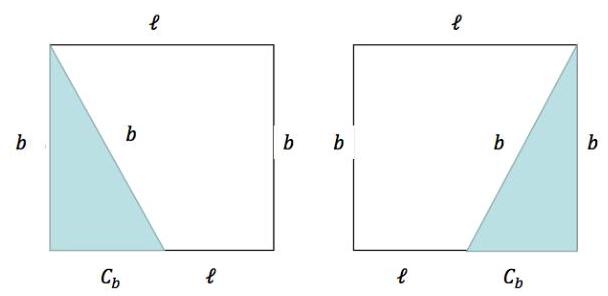
\includegraphics[width=0.65\textwidth]{images/Ch7_identity_pi1.jpg}
\end{center}
4. Inverse: the inverse of \(\left\lbrack  u\right\rbrack\), where \(u\) is a loop, should be \(\left\lbrack  {u}^{\prime }\right\rbrack\), where \({u}^{\prime }\) is the reverse of the traveling of \(u\). More explicitly, for all loop \(u : I \rightarrow  X\) based at \(b\), define \({u}^{-1} : I \rightarrow  X\) by \({u}^{-1}\left( t\right)  = u\left( {1 - t}\right)\). Note that
\[
\left\lbrack  u\right\rbrack   * \left\lbrack  {u}^{-1}\right\rbrack   = \left\lbrack  {u \cdot  {u}^{-1}}\right\rbrack ,\;e = \left\lbrack  {c}_{b}\right\rbrack
\]
So it suffices to show \(u \cdot  {u}^{-1} \simeq  {c}_{b}\) and \({u}^{-1} \cdot  u \simeq  {c}_{b}\) :

The homotopy below gives \(u \cdot  {u}^{-1} \simeq  {c}_{b}\).
\[
H\left( {t,s}\right)  = \left\{  \begin{array}{rr} u\left( {{2t}\left( {1 - s}\right) }\right), & 0 \leq  t \leq  1/2 \\  u\left( {\left( {2 - {2t}}\right) \left( {1 - s}\right) }\right), & 1/2 \leq  t \leq  1 \end{array}\right.
\]
The graphic illustration is given below:
\begin{center}
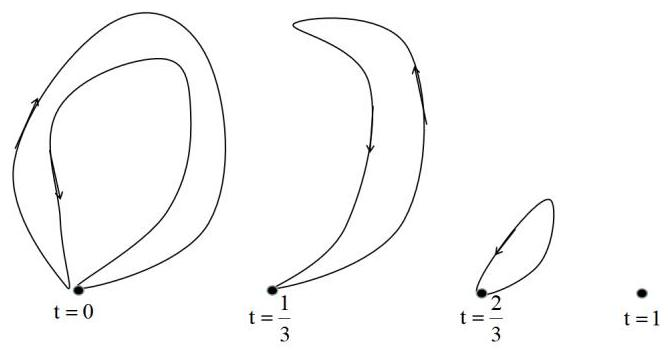
\includegraphics[width=0.5\textwidth]{images/Ch7_inverse_pi1.jpg}
\end{center}
So the result follows.
\end{proof}

\begin{remark}
Note that the figure below does not define a homotopy from \(u \cdot  {u}^{-1}\) to \({c}_{b}\):
\begin{center}
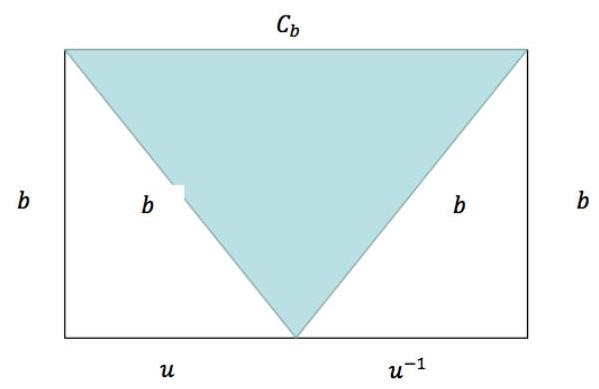
\includegraphics[width=0.5\textwidth]{images/Ch7_inverse_countereg_pi1.jpg}
\end{center}
The reason is that when we move from bottom to above in the figure, i.e. \(s \rightarrow  1\), if we look at the white triangles, the time to travel along \(u\) and \({u}^{-1}\) reduces from $1/2$ seconds to $0$ second. In other words, when $s \to 1$ one has to go along \(u\) and \({u}^{-1}\) at infinite speed, and hence it is not well-defined. 

As an exercise, try to write down the function $H:[0,1] \times [0,1] \to X$ explicitly for the above diagram, and check that $H(t,s) \to \infty$ as $s \to 1$.
\end{remark}

\begin{example} We now check \({\pi }_{1}\left( {{\mathbb{R}}^{2},b}\right)  = \{ e\}\) is trivial: For any \(u : I \rightarrow  {\mathbb{R}}^{2}\) with \(u\left( 0\right)  = u\left( 1\right)  = b\), consider the homotopy
\[
H\left( {t,s}\right)  = \left( {1 - s}\right) u\left( t\right)  + {sb}.
\]
Therefore, \(u \simeq  {c}_{b}\) for any loop \(u\) based at \(b\). 

Check the diagram below for graphic illustration of this homotopy.
\begin{center}
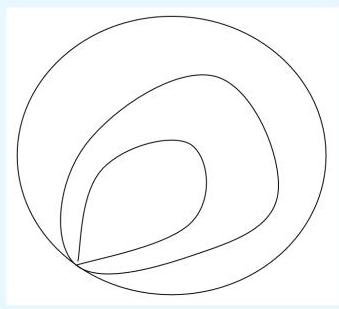
\includegraphics[width=0.4\textwidth]{images/Ch7_R2_trivial_pi1.jpg}
\end{center}

More generally, if \(X \simeq  \{ x\}\) is contractible, then \({\pi }_{1}\left( {X,b}\right)  = \{ e\}\). The same argument cannot work for \(\left( {{\mathbb{R}}^{2} \backslash \{ 0\},\mathbf{b}}\right)\), since the mapping \(H : {\mathbb{R}}^{2} \smallsetminus  \{ 0\}  \times  I \rightarrow  {\mathbb{R}}^{2} \smallsetminus  \{ 0\}\) with
\(H\left( {\mathbf{t},s}\right)  = \left( {1 - s}\right) u\left( \mathbf{t}\right)  + s\mathbf{b}\) is not well-defined. In particular, the value \(H\left( {s,t}\right)\) may hit the origin 0.
\end{example}

\begin{proposition} \label{prop:path_connected_isomotphic} If \(b,{b}^{\prime }\) are path-connected in \(X\), then \({\pi }_{1}\left( {X,b}\right)  \cong  {\pi }_{1}\left( {X,{b}^{\prime }}\right)\).
\end{proposition}

\begin{proof} Let \(w\) be a path from \(b\) to \({b}^{\prime }\), and define
\[
{w}_{\# } : \;{\pi }_{1}\left( {X,b}\right)  \rightarrow  {\pi }_{1}\left( {X,{b}^{\prime }}\right)
\quad
\text{ with }\left\lbrack  \ell \right\rbrack   \mapsto  \left\lbrack  {{w}^{-1}\ell w}\right\rbrack.
\]
1. \({w}_{\# }\) is well-defined: Check that \(\ell  \simeq  {\ell }^{\prime }\) implies \({w}^{-1}\ell w \simeq  {w}^{-1}{\ell }^{\prime }w\). See the figure below for graphic illustration.
\begin{center}
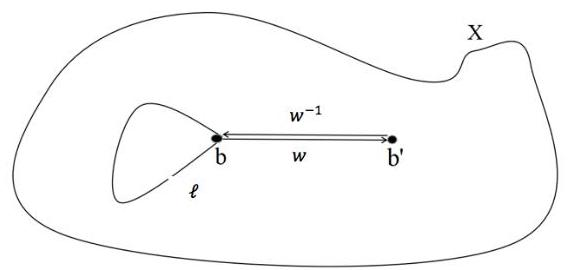
\includegraphics[width=0.5\textwidth]{images/Ch7_path_connected.jpg}
\end{center}
2. \({w}_{\# }\) is a homomorphism:
\[
{w}_{\# }\left( \left\lbrack  {\ell }_{1}\right\rbrack  \right)  \cdot  {w}_{\# }\left( \left\lbrack  {\ell }_{2}\right\rbrack  \right)  = \left\lbrack  {{w}^{-1} \cdot  {\ell }_{1}w}\right\rbrack   \cdot  \left\lbrack  {{w}^{-1} \cdot  {\ell }_{2}w}\right\rbrack   = \left\lbrack  {{w}^{-1} \cdot  {\ell }_{1}{\ell }_{2}w}\right\rbrack  = {w}_{\# }\left( \left\lbrack  {{\ell }_{1}{\ell }_{2}}\right\rbrack  \right)  
\]
where the second equality is due to the fact that \(w \cdot  {w}^{-1} \simeq {c}_{b}\).

3. \({w}_{\# }\) is injective: If the loops \({\ell }_{1},{\ell }_{2}\) are such that \({w}_{\# }\left( {\ell }_{1}\right)  = {w}_{\# }\left( {\ell }_{2}\right)\), i.e.
\[
\left\lbrack  {{w}^{-1}{\ell }_{1}w}\right\rbrack   = \left\lbrack  {{w}^{-1}{\ell }_{2}w}\right\rbrack
\]
Extend the definition of \(\left\lbrack  \ell \right\rbrack\) to allow \(\ell\) to be a path, and the equivalence class is defined by the relation " \(\sim\) ": \({\ell }_{1} \sim  {\ell }_{2}\) iff they are homotopic relative to \(\{ 0,1\}\), then
\[
\left\lbrack  {\ell }_{1}\right\rbrack   = \left\lbrack  w\right\rbrack  \left\lbrack  {{w}^{-1}{\ell }_{1}w}\right\rbrack  \left\lbrack  {w}^{-1}\right\rbrack   = \left\lbrack  w\right\rbrack  \left\lbrack  {{w}^{-1}{\ell }_{2}w}\right\rbrack  \left\lbrack  {w}^{-1}\right\rbrack   = \left\lbrack  {\ell }_{2}\right\rbrack   \tag{11.5}
\]

4. \({w}_{\# }\) is surjective: we give the inverse of \({w}_{\# }\) explicitly:
\[
{w}_{\# }^{-1} : \;{\pi }_{1}\left( {X,{b}^{\prime }}\right)  \rightarrow  {\pi }_{1}\left( {X,b}\right)
\quad \text{ with }\left\lbrack  m\right\rbrack   \mapsto  \left\lbrack  {w \cdot  m \cdot  {w}^{-1}}\right\rbrack
\]
\end{proof}

From now on, for any path connected space \(X\), we will just write \({\pi }_{1}\left( X\right)\) instead of \({\pi }_{1}\left( {X,x}\right)\) if it causes no confusion.

\begin{proposition} \label{prop:pi1_homomorphism} Let $(X, x)$ and $(Y, y)$ be topological spaces with basepoints \(x\) and \(y\), and \(f : X \rightarrow  Y\) be a continuous map with \(f\left( x\right)  = y\). Then every loop \(\ell  : I \rightarrow  X\) based at \(x\) gives a loop \(f \circ  \ell  : I \rightarrow  Y\) based at \(y\), i.e., the continuous map \(f\) induces a homomorphism of groups
\[
{f}_{ * } : \;{\pi }_{1}\left( {X,x}\right)  \rightarrow  {\pi }_{1}\left( {Y,y}\right),
\quad \quad
\left\lbrack  \ell \right\rbrack   \mapsto  \left\lbrack  {f \circ  \ell }\right\rbrack   \mathrel{\text{ := }} {f}_{ * }\left( \left\lbrack  \ell \right\rbrack  \right)
\]
Moreover,

1. \({\left( {\operatorname{id}}_{X \rightarrow  X}\right) }_{ * } = {\operatorname{id}}_{{\pi }_{1}\left( {X,x}\right)  \rightarrow  {\pi }_{1}\left( {X,x}\right) }\)

2. \({\left( g \circ  f\right) }_{ * } = {g}_{ * } \circ  {f}_{ * }\)

3. If \(f \simeq  {f}^{\prime }\) relative to \(x \in  X\), then \({f}_{ * } = {\left( {f}^{\prime }\right) }_{ * }\)
\end{proposition}

\begin{proof}
Well-definedness: Suppose that \(\ell  \simeq  {\ell }^{\prime }\), then \(f \circ  \ell  \simeq  f \circ  {\ell }^{\prime }\) by \autoref{prop:comp_homotopy}.
Therefore, \(\left\lbrack  {f \circ  \ell }\right\rbrack   = \left\lbrack  {f \circ  {\ell }^{\prime }}\right\rbrack\).

Homomorphism: It is clear that
\[
f \circ  \left( {\ell  \circ  {\ell }^{\prime }}\right)  = \left( {f \circ  \ell }\right)  \circ  \left( {f \circ  {\ell }^{\prime }}\right)
\]
Therefore, \({f}_{ * }\left\lbrack  {\ell {\ell }^{\prime }}\right\rbrack   = \left( {{f}_{ * }\left\lbrack  \ell \right\rbrack  }\right)  * \left( {{f}_{ * }\left\lbrack  {\ell }^{\prime }\right\rbrack  }\right)\)
The other three statements are obvious.
\end{proof}

\begin{proposition} \label{prop:homotopy_equiv_isomorphism} Let \(X,Y\) be path-connected such that \(X \simeq  Y\) are homotopy equivalent (i.e., there exists \(f : X \rightarrow  Y\) and \(g : Y \rightarrow  X\) such that \(g \circ  f \simeq  {\operatorname{id}}_{X},f \circ  g \simeq  {\operatorname{id}}_{Y}\) ). Then 
\[{\pi }_{1}\left( X\right)  \cong  {\pi }_{1}\left( Y\right).\]
In particular, if \(X,Y\) are path-connected such that \(X \cong  Y\) are homeomorphic, then \({\pi }_{1}\left( X\right)  \cong  {\pi }_{1}\left( Y\right)\).
\end{proposition}

\begin{proof} Consider the mapping
\[
{\pi }_{1}\left( {X,{x}_{0}}\right) \overset{{f}_{ * }}{ \rightarrow  }{\pi }_{1}\left( {Y,{y}_{0}}\right) \overset{{g}_{ * }}{ \rightarrow  }{\pi }_{1}\left( {X,{x}_{1}}\right)
\]
By \autoref{prop:pi1_homomorphism}, \({f}_{ * }\) and \({g}_{ * }\) are homomorphisms. So it suffices to show that \({f}_{ * }\) and \({g}_{ * }\) are bijective.

{\bf Wrong proof:} \(g \circ  f \simeq  {\operatorname{id}}_{X}\) implies \({\left( g \circ  f\right) }_{ * } = {\left( {\operatorname{id}}_{X}\right) }_{ * }\) implies \({g}_{ * } \circ  {f}_{ * } = {\operatorname{id}}_{{\pi }_{1}\left( {X,{x}_{0}}\right) }\).

{\bf Reason:} \(\left( {g \circ  f}\right)  \simeq  {\operatorname{id}}_{X}\) is not relative to \({x}_{0}\).

So we have to work harder -- Consider the homotopy \(H : g \circ  f \simeq  {\mathrm{{id}}}_{X}\), where \(H\left( {{x}_{0},s}\right)\) is not necessarily a constant for \(s \in  I\). It follows that \(H\left( {{x}_{0},0}\right)  = {x}_{1}\) and \(H\left( {{x}_{0},1}\right)  = {x}_{0}\), i.e., \(w\left( s\right)  \mathrel{\text{ := }} H\left( {{x}_{0},s}\right)\) defines a path from \({x}_{1}\) to \({x}_{0}\).

For any loop \(\ell  : I \rightarrow  X\) based at \({x}_{0}\), consider the homotopy
\[
K = H \circ  \left( {\ell  \times  {\operatorname{id}}_{I}}\right)  : \;I \times  I \rightarrow  X
\]
given by
\begin{align*}
K\left( {t,s}\right)  &= H\left( \left( {\ell \left( t\right),s}\right) \right) \\
K\left( {t,0}\right)  &= H\left( {\ell \left( t\right),0}\right)  = g \circ  f\left( {\ell \left( t\right) }\right)
\\
K\left( {t,1}\right) &= H\left( {\ell \left( t\right),1}\right)  = \ell \left( t\right)
\\
K\left( {0,s}\right)  &= w\left( s\right)  = K\left( {1,s}\right)
\end{align*}
The graphic plot of \(K\) is given in the figure below:
\begin{center}
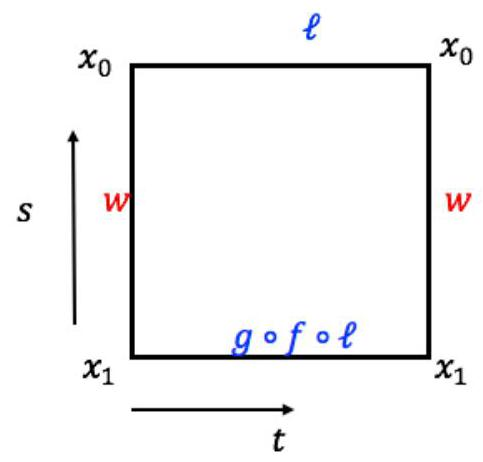
\includegraphics[width=0.4\textwidth]{images/Ch7_K_homotopy.jpg}
\end{center}

The homotopy $K$ between \(\ell\) and \(g \circ  f \circ  \ell\) is not relative to $\{0,1\}$. But we can modify it to get a homotopy between \(\ell\) and \({w}^{-1} \circ  g \circ  f \circ  \ell  \circ  w\) relative to \(\{ 0,1\}\) :
\begin{center}
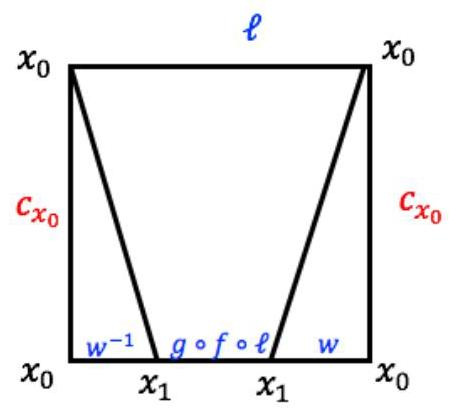
\includegraphics[width=0.4\textwidth]{images/Ch7_K_homotopy_2.jpg}
\end{center}
Therefore,
\[
\left\lbrack  \ell \right\rbrack   = \left\lbrack  {{w}^{-1}{gf}\ell w}\right\rbrack   = {w}_{\# }\left( \left\lbrack  {{gf}\ell }\right\rbrack  \right)  = \left( {{w}_{\# } \circ  {g}_{ * } \circ  {f}_{ * }}\right) \left\lbrack  \ell \right\rbrack
\]
which follows that \({w}_{\# } \circ  {g}_{ * } \circ  {f}_{ * } = {\operatorname{id}}_{{\pi }_{1}\left( {X,{x}_{0}}\right) }\). By \autoref{prop:path_connected_isomotphic}, ${w}_{\# }: \pi_1(X,x_0) \to \pi_1(X,x_1)$ is a group isomorphism. Therefore, \({f}_{ * }\) is injective, \({g}_{ * }\) is surjective.

Similarly, one can modify the above argument and get
\[
{w}_{\# } \circ  {f}_{ * } \circ  {g}_{ * } = {\operatorname{id}}_{{\pi }_{1}\left( {Y,{y}_{0}}\right) }
\]
Therefore, \({f}_{ * }\) is surjective, \({g}_{ * }\) is injective, and the result follows.
\end{proof}

\begin{definition} \label{def:simply_connected} [Simply-Connected] A space \(X\) is \emph{simply-connected} if \(X\) is path connected, and \(X\) has trivial fundamental group, i.e., \({\pi }_{1}\left( X\right)  = \{ e\}\) for some point \(e \in  X\).
\end{definition}
\begin{example} If \(X\) is contractible, then \(X \simeq  \{ x\}\) is simply-connected. Indeed, \autoref{prop:homotopy_equiv_isomorphism}, 
\[
{\pi }_{1}\left( X\right)  \cong  {\pi }_{1}\left( {\{ x\} }\right)  = \{ e\}.
\]
Therefore, all contractible spaces (e.g. \({\mathbb{R}}^{n}\) ) are simply-connected.
\end{example}

However, not all simply-connected spaces are contractible, e.g., \({\pi }_{1}\left( {S}^{2}\right)  \cong  \{ e\}\), but \({S}^{2}\) is not homotopy equivalent to a point.